\documentclass[12pt, twosided]{article}

\usepackage[letterpaper,bindingoffset=0in,%
            left=1in,right=1in,top=1in,bottom=1in,%
            footskip=.25in]{geometry}

\usepackage{mathtools}
\usepackage{graphicx}

\usepackage{setspace}
\setstretch{1.1}

\usepackage{amsmath}
\usepackage{amsfonts}
\usepackage{amsthm}
\usepackage{amssymb}
\usepackage{csquotes}
\usepackage{relsize}

\usepackage{tikz}
\usetikzlibrary{cd}
\usetikzlibrary{fit,shapes.geometric}
\tikzset{%  
    mdot/.style={draw, circle, fill=black},
    mset/.style={draw, ellipse, very thick},
}

\usepackage{hhline}
\usepackage{systeme}
\usepackage{mathrsfs}
\usepackage{hyperref}
\usepackage{mathtools}  
\usepackage{silence}
\usepackage{blkarray}
\usepackage{float}
\usepackage{framed}
\usepackage{array}
\usepackage{stmaryrd}
\usepackage{extarrows}
\usepackage{caption}
\captionsetup[figure]{labelfont={bf},name={Fig.},labelsep=period}

\theoremstyle{definition}
\newtheorem{df}{Definition}
\newtheorem{exa}{Example}
\newtheorem{ques}{Question}
\newtheorem{exr}{Exercise}
\newtheorem*{note}{Note}
\theoremstyle{plain}
\newtheorem{thm}{Theorem}
\newtheorem{prop}{Proposition}
\newtheorem{conj}{Conjecture}
\newtheorem{cor}{Corollary}
\newtheorem{lm}{Lemma}
\newtheorem*{fact}{Fact}
\newtheorem*{idea}{Idea}
\newtheorem*{clm}{Claim}
\newtheorem*{rmk}{Remark}
\usepackage[ruled]{algorithm2e}

\usepackage{ulem}
\makeatletter

\def\lf{\left\lfloor}   
\def\rf{\right\rfloor}
\def\lc{\left\lceil}   
\def\rc{\right\rceil}
\def\st{\text{ s.t. }}
\def\1{^{-1}}
\def\ind{\mathbf{1}}
\def\R{\mathbb{R}}
\def\Q{\mathbb{Q}}
\def\Z{\mathbb{Z}}
\def\C{\mathbb{C}}
\def\I{\mathbb{I}}
\def\N{\mathbb{N}}
\def\F{\mathbb{F}}
\def\A{\mathbb{A}}
\def\Li{\text{Li}}
\def\th{^\text{th}}
\def\sp{\text{Sp}}
\def\opn{\left\{}
\def\cls{\right\}}
\def\Aut{\text{Aut}}
\def\PG{\text{PG}}
\def\GL{\text{GL}}
\def\PGL{\text{PGL}}
\def\Cov{\text{Cov}}
\def\Pack{\text{Pack}}
\def\PgamL{\text{P}\Gamma\text{L}}
\def\gamL{\Gamma\text{L}}
\def\cl{\text{cl}}
\def\stbar{\ \middle\vert\ }
\def\partdone{\hphantom{1} \hfill \(\triangle\)}
\def\s0{_0}
\def\s1{_1}
\def\s2{_2}
\def\id{\mathrm{id}}
\def\topn{\text{ open}}
\def\Bd{\text{Bd }}
\renewcommand{\P}{\mathbb{P}}
\newcommand{\leg}[2]{\left( \frac{#1}{#2} \right)}
\renewcommand*\env@matrix[1][*\c@MaxMatrixCols c]{%
   \hskip -\arraycolsep
   \let\@ifnextchar\new@ifnextchar
   \array{#1}}
\makeatother

% These two lines suppress the warning generated 
% by amsmath for overwriting the choose command  
% because it's annoying. This probably has unint-
% ended ramifications somewhere else, but I'm too
% lazy to actually figure that out, so we'll cro-
% ss that bridge when we come to it lol.
\renewcommand{\choose}[2]{\left( {#1 \atop #2} \right)}
\WarningFilter{amsmath}{Foreign command} 

\renewcommand{\mod}[1]{\ (\mathrm{mod}\ #1)}
\renewcommand{\vec}[1]{\mathbf{#1}}

\let\oldprime\prime
\def\prime{^\oldprime}

\usepackage{float}
\restylefloat{figure}

\usepackage{cleveref}
\Crefname{thm}{Theorem}{Theorems}

% Comment commands for co-authors
\newcommand{\kmd}[1]{{\color{purple} #1}}

\newcolumntype{L}{>{$}l<{$}}
% Bib matter
\let\oldepsilon\epsilon
\def\epsilon{\varepsilon}

\let\oldphi\phi
\def\phi{\varphi}

%%% Local Variables:
%%% mode: plain-tex
%%% TeX-master: t
%%% End:

\graphicspath{{./img/}}

\begin{document}
\noindent \textbf{Math 171} \hfill \textbf{Professor Sebastian Bozlee} \\
\textbf{Scribed by: Kyle Dituro} \hfill \textbf{\(\pi\), 2023}\hrule
\vspace{.2in}

We recall the definition of the product topology:

\begin{df}
  Let \(X , Y\) be topological spaces. Then the \textbf{product topology} is the topology on \(X \times Y\) generated by the basis:
  \begin{align*}
    \mathcal{B} = \opn U \times V \stbar U \subseteq X\ \mathrm{open},\ V \subseteq Y\ \mathrm{open} \cls.
  \end{align*}
\end{df}

\begin{exa}
  \(\R^2\) has the product topology induced by thinking of \(\R^2\) as \(\R\times \R\).

  \begin{figure}[h]
    \centering
    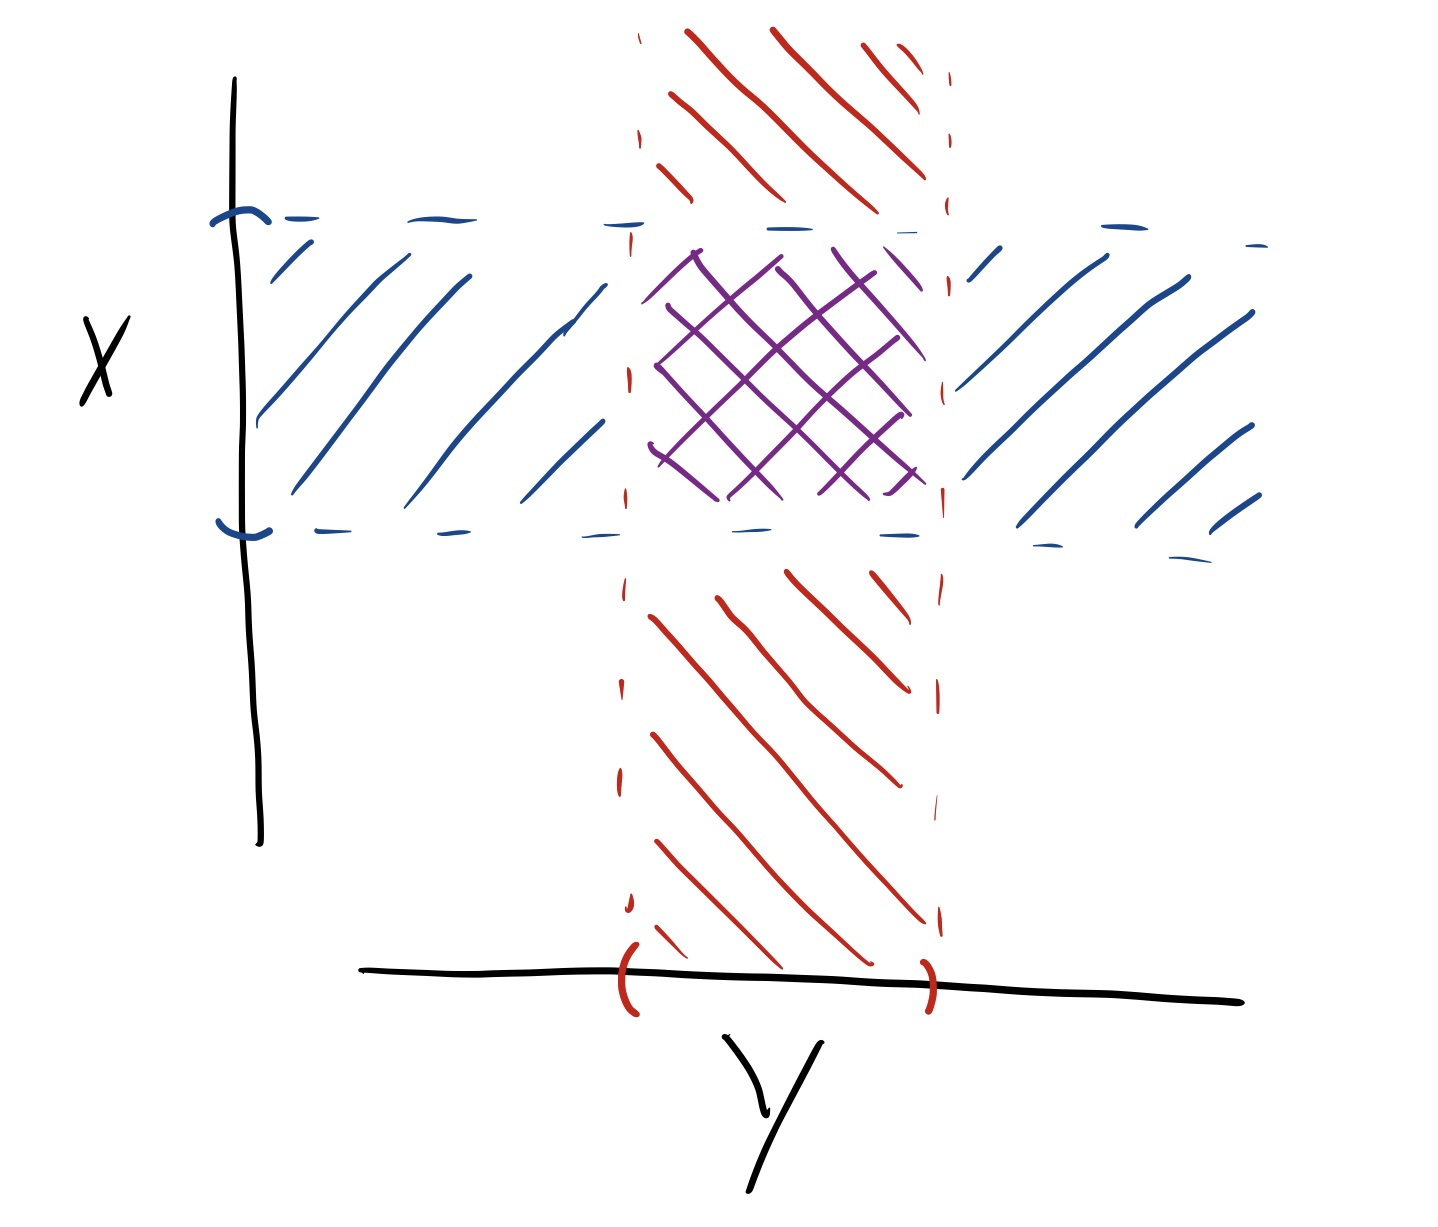
\includegraphics[width=.5\textwidth]{ProductTop}
    \caption{Basis by open rectangles}
    \label{fig:dubious}
  \end{figure}
\end{exa}

\begin{fact}
  If \(\mathcal{B}_X\) and \(\mathcal{B}_Y\) are bases for \(X, Y\), then
  \begin{align*}
    \mathcal{B} = \opn B_X \times B_Y \stbar B_X \in \mathcal{B}_X, B_Y \in \mathcal{B}_Y \cls
  \end{align*}
  is also a basis for the product topology.
\end{fact}

\begin{prop}
  The set
  \begin{align*}
    \opn U \times V \stbar U \subseteq X\ \mathrm{open}, V \subseteq Y\ \mathrm{open} \cls
  \end{align*}
  really is a basis.
\end{prop}

\begin{proof}
  \begin{enumerate}
  \item \textit{(Each point belongs to a basis element)} Let \((x, y) \in X \times Y\). Then \((x, y) \in X \times Y\), and \(X \subseteq X\) is open, \(Y \subseteq Y\) is open, so we have a basis element containing \((x, y)\).
  \item Let \(B_1 = U_1 \times V_1\), \(B_2 = U_2 \times V_2\), where the \(U_i\) are open in \(X\), and \(V_j\) are open in \(Y\). Then

    \begin{align*}
      B_1 \cap B_2 &= (U_1 \times V_1) \cap (U_2 \times V_2) \\
                   &= \opn (x, y) \in X \times Y \stbar x \in U_1 \wedge y \in V_1 \cls \cap \opn (x, y) \in X \times Y \stbar x \in U_2 \wedge y \in V_2 \cls \\
                   &= \opn (x, y) \in X \times Y \stbar (x \in U_1) \wedge (x \in U_2) \wedge (y \in V_1) \wedge (Y \in V_2) \cls \\
                   &= \opn (x, y) \in X \times Y \stbar (x \in U_1 \cap U_2) \wedge (y \in V_1 \cap V_2) \cls \\
                   &= (U_1 \cap U_2) \times (V_1 \cap V_2)
    \end{align*}
    This is a basis element, so for any \((x, y) \in B_1 \cap B_2\) we can set \(B_3 = B_1 \cap B_2\) to satisfy the axiom.
  \end{enumerate}
\end{proof}

\begin{thm}
  Let \(X, Y\) be topological spaces.
  \begin{enumerate}
  \item The product topology on \(X \times Y\) is the coarsest topology such that
    \begin{align*}
      \begin{matrix}
        \pi_1: X \times Y \to X \\ (x, y) \mapsto x
      \end{matrix} \quad\quad
      \begin{matrix}
        \pi_2: X \times Y \to Y \\ (x, y) \mapsto y
      \end{matrix}
    \end{align*} are continuous functions.
  \end{enumerate}
\item \(X \times Y\) with the product topology and \(\pi_1, \pi_2\) have the universal property of the product for topological spaces.
\end{thm}
\begin{proof}
  \begin{enumerate}
  \item Recall: \(\pi_1\) is continuous iff for all \(U \subseteq X\) open, we have that \(\pi_1\1(U = U \times Y)\) is open. Similarly for \(\pi_2\), we need tat for all \(V \subseteq Y\) open, we have that \(\pi_1\1(V) = X \times V\) is open. These are open in the product topology so \(\pi_1, \pi_2\) are continuous. To complete the proof, suppose that \(\tau\) is a topology on \(X \times Y\) such that \(\pi_1, \pi_2\) are continuous.  Then for all \(U \subseteq X\) open, \(V \subseteq Y\) open, we have that \(U \times Y\) and \(X \times V\) are open. Then intersection \((U \times Y) \cap (X \times V) = (U \cap X) \times (Y \cap V) = U \times V\) is open as well.

    Then since \(\tau\) contains the basis for the product topology, we proved on the HW that \(\tau\) contains the product topology too.
  \item Now let's show that we have the universal property of the product. We need to show that for all diagrams of topological spaces
    \begin{center}
      \begin{tikzcd}
        & Z \arrow[dr, "f_2"] \arrow[d, "\exists! f"] & \\
        X \arrow[leftarrow, ur, "f_1"] & X \times Y \arrow[l, "\pi_1"] & Y \arrow[leftarrow, l, "\pi_2"]
      \end{tikzcd}
    \end{center}
    
  there is a unique continuous function \(f\) such that the diagram commutes. By the universal property of products of sets, there is a unique function \(f: Z \to X \times Y\) making the diagram commute, namely \(z \mapsto (f_1(z), f_2(z))\). It suffices to show that this \(f\) is continuous.

  By HW, it suffices to show \(f\1(B)\) is open for each basic open set in the product topology.

  Let \(B = U \times V\) be a basis element, where \(U \subseteq X\) open \(V \subseteq Y\) open. Then

  \begin{align*}
    f\1(B) &= \opn z \in Z \stbar f(z) \in B \cls \\
           &= \opn z \in Z \stbar (f_1(z), f_2(z)) \in U \times V \cls \\
           &= \opn z \in Z \stbar f_1(z) \in U\ \mathrm{and}\ f_2(z) \in V \cls \\
           &= \opn z \in Z \stbar f_1(z) \in U \cls \cap \opn z \in Z \stbar f_1(z) \in V \cls \\
           &= \underbrace{\underbrace{f\1_1(U)}_{\mathrm{open}} \cap \underbrace{f_2\1(V)}_{\mathrm{open}}}_{\mathrm{open}}
  \end{align*}
\end{enumerate}
\end{proof}

\begin{cor}[Universal property, short version]
  If \(f_1: Z \to X\) and \(f_2: Z \to Y\) are continuous functions, then
  \begin{align*}
    f_1 \times f_2: &Z \to X \times Y \\
                    &z \mapsto (f_1(z), f_2(z))
  \end{align*}
  is continuous too.
\end{cor}

\begin{exa}
  \(\R^{n_1 + n_2}\) has the universal property of the product induced by thinking of \(\R^{n_1 + n_2}\) as \(\R^{n_1} \times \R^{n_2}\) . Therefore \(\R^{n_1 + n_2}\) has the product topology.
\end{exa}
Let's give one final lemma which should illustrate how we reason about the product topology.

\begin{lm}
  Let \(X, Y\) be topological spaces. Let \(Z \subseteq X\) and \(W \subseteq Y\) be closed subsets. Then \(Z \times W \subseteq X \times Y\) is closed.
\end{lm}

\begin{proof}
  We want to show that \((Z \times W)^c\) is open in the product topology. Notice that \((Z \times W)^c = \underbrace{(Z^c \times Y)}_{\mathrm{open}} \cap \underbrace{(X \times W^c)}_{\mathrm{open}}\). So \((Z \times W)^c\) is open, as desired.
\end{proof}

\begin{ques}
  What about more spaces? \(X_1 \times \ldots \times X_n\) should have the topology generated by \(U_1 \times \ldots U_n\).

  \(\prod_{i \in I} X_i\) should have the topology generated by \(\prod_{i \in I} U_i\) where the \(U_i\) are open for each \(i\), and \(U_i = X_i\) \textit{for all but finitely many \(i\)}.
\end{ques}
\end{document}
%%% Local Variables:
%%% mode: latex
%%% TeX-master: t
%%% End:
